\documentclass[a4paper, 14pt]{extarticle}
% \documentclass{article}

\usepackage{graphicx}%Вставка картинок правильная
\usepackage{float}%"Плавающие" картинки
\usepackage{wrapfig}%Обтекание фигур (таблиц, картинок и прочего)
\usepackage[utf8]{inputenc}
\usepackage[T2A]{fontenc}
\usepackage[unicode, pdftex]{hyperref}
\usepackage[english,russian]{babel}
\usepackage[autostyle]{csquotes}
\usepackage{multirow}
\usepackage{adjustbox}


\usepackage[left=30mm, top=25mm, right=15mm, bottom=25mm]{geometry}
\linespread{1.3}
\pagenumbering{arabic}

\begin{document}
    \begin{center}
      \hfill \break 
      \small{Федеральное государственное автономное образовательное\\ учреждение высшего образования}\\ 
        \vspace{0.5ex}
      \textbf{\small{<<НАЦИОНАЛЬНЫЙ ИССЛЕДОВАТЕЛЬСКИЙ УНИВЕРСИТЕТ\\ <<ВЫСШАЯ ШКОЛА ЭКОНОМИКИ>>}}\\
        \vspace{0.5ex}
      \small{\textbf{Факультет компьютерных наук}}\\
        \vspace{13ex}
      \textbf{\normalsize{КУРСОВАЯ РАБОТА}}\\
      \hfill \break
      \normalsize{Разработка алгоритма расчета индекса этичности компании на основе текстовых открытых данных }\\
      \hfill \break
      \small{по направлению подготовки Прикладная математика и информатика\\ образовательная программа <<Финансовые технологии и анализ данных>>}\\
    \end{center}
    
    \vspace{9ex}
    
    \begin{flushright} % выравнивание по правому краю
      \begin{minipage}{0.4\textwidth} % врезка в половину ширины текста
        \begin{flushleft} % выровнять её содержимое по левому краю
          
          \small\textbf{Работу выполнил:}\\
          \small Студент группы мФТиАД22 \\
          \small Ященко Михаил Андреевич\\
          \hspace{0.2mm} \\
          \underline{\hspace{6cm}} \\

          \hspace{2cm} \\
          
          \small \textbf{Научный руководитель:}\\
          \small Кандидат экономических наук \\
          \small Сторчевой Максим Анатольевич \\
          \hspace{0.2mm} \\
          \underline{\hspace{6cm}} \\
          
          
        \end{flushleft}
      \end{minipage}
    \end{flushright}
    \vfill
    \begin{center} \small Москва 2023 \end{center}
    \thispagestyle{empty} % выключаем отображение номера для этой страницы
    % КОНЕЦ ТИТУЛЬНОГО ЛИСТА

\newpage
\setcounter{page}{2}
\section*{Аннотация}
Сейчас, когда говорят о оценке этичности компаний, чаще всего речь идет про ESG. Это важно, для снижения рисков, как самих компаний, так и их клиентов, улучшения репутации компании: если компания придерживается принципов ESG, это может привлечь привлечь больше инвесторов и партнеров. Также ESG оценивает, как компании влияют на качество жизни людей и общества в целом, и окржуающую среду. На данный момент есть несколько рейтитингов ESG. Но с этими рейтингами есть ряд проблем: рейтинги не всегда согласуются между собой из-за разных методик оценки, чаще всего это трудоемкая ручная работа, требующая много часов, в текущих рейтингах не так много компаний. Поэтому встал вопрос об автоматизации расчета индекса этичности компаний. Для этого мы решили использовать нефинансовые отчеты компаний с сайта РСПП и на их основе разработать собственный алгоритм расчета показателей ESG.
\newline
\newline
Now, when we talk about assessing the ethics of companies, most often we are talking about ESG. This is important to reduce the risks of both the companies themselves and their customers, to improve the reputation of the company: if the company adheres to the principles of ESG, it can attract more investors and partners. ESG also assesses how companies affect the quality of peoples life and society, and the environment. There are several ESG ratings at the moment. But there are a number of problems with these ratings: they do not always agree with each other due to different evaluation methods, most often it is laborious manual work that requires many hours, there are not so many companies in the current ratings. Therefore, the question arose about automating the calculation of the ethics index of companies. To do this, we decided to use non-financial reports of companies from the RSPP website and develop our own algorithm for calculating ESG indicators based on them.

% СОДЕРЖАНИЕ
\newpage
\setcounter{page}{3}

\tableofcontents

\newpage
\setcounter{page}{4}
\pagestyle{plain}
\section{Введение}
ESG (от английского Environmental, Social, and Corporate Governance — экология, общество и корпоративное управление) --- это концепция, которая включает в себя три аспекта устойчивого развития: забота об окружающей среде, социальная ответственность и корпоративное управление. Есть несколько причин, почему ESG это важно:
\begin{itemize}
    \item Снижение рисков: ESG-рейтинги помогают компаниям оценить свои риски и возможности, связанные с экологическими, социальными и управленческими аспектами своей деятельности. Это может помочь компаниям принимать более обоснованные решения и снизить риски для себя и для окружающей среды.
    \item Улучшение репутации: компании, которые придерживаются принципов ESG, могут улучшить свою репутацию и привлечь больше инвесторов и партнеров. Это может привести к увеличению прибыли и росту бизнеса.
    \item Влияние на общество: ESG-принципы направлены на то, чтобы компании учитывали интересы своих сотрудников, клиентов, партнеров и общества в целом. Соблюдение этих принципов может привести к улучшению качества жизни людей и уменьшению негативного влияния на окружающую среду.
    \item Повышение устойчивости: ESG-подход помогает компаниям стать более устойчивыми к изменениям в мировой экономике и обществе. Это может снизить зависимость от краткосрочных финансовых результатов и повысить долгосрочную устойчивость бизнеса.
\end{itemize}

На сегодняшний день рейтинги и индексы этичности ESG формируются различными организациями, такими как рейтинговые агентсва, банки, инвестиционные фонды и другие финансовые институты. Они используют различные методики оценки, учитывают много разных факторы, из-за чего итоговые результаты не всегда совпадают. Сейчас это делается в ручную, это сложная трудоемкая работа, которая отнимает много времени и ресурсов.

Данный проект призван автоматизировать часть этой работы связанную с выделением фактором из нефинансовых отчетов компаний.

Результатом данной работы стал алгоритм для оценки покрытия нефинансового отчета подтопиками ESG с дальнейшим получением индекса этичности на основе этой оценки. Полученный индекс сравнивался с рейтингами RAEX \cite{link:raex-methodik} и РСПП \cite{link:rspp-methodik}. 

\section{Цели и задачи проекта}
Целью данного проекта было получение алгоритма, который автоматически на основе нефинансового отчета компании, оценивает насколько компания соответсвует концепции устойчивого развития ESG. Отмечу, что мы не можем дать полную оценку только на основе нефинансовых отчетов, так как компании не пишут о себе плохо в отчетах. Но мы можем оценить открытость организации и то, насколько она раскрывает данные о своей деятельности.

После этого необходимо сравнить индекс получнный алгоритмом с уже известными рейтингами и проанализировать полученные результаты.

\section{План выполнения проекта}
\subsection{Предобоработка корпуса нефинансовых отчетов}

В качестве выборки мы использовали корпус нефинансовых отчетов, который есть на сайте Российского союза
промышленников и предпринимателей в свободном доступе. Всего там представлено 1388 отчетов разных компаний за разные года с укзанием типа отчета (отчет по устойчивому развитию, социальный отчет, интегрированный отчет, экологический отчёт), сектора, в котором работает компания (образование, здравоохранение, энергетика и т.д.). 

После скачивание отчетов в формате PDF с сайта РСПП, они были распарсены по страницам в тексты, были убраны знаки препинания, и оставлены только слова на кириллице. Затем все слова были лемматизированы. После мы посчитали сколько раз каждое слово используется в отчете, и в каком количестве отчетов оно встречается. На основе этой статистики мы убрали слова, которые встречаются слишком редко или слишком часто. В итоге из страниц нефинансовых отчетов получился корпус текстов, которые в дальнейшем использовались в качестве обучающей выборки для модели Top2Vec.  

\subsection{Выделение топиков моделью Top2Vec}

На основе полученного корпуса текстов мы выделили топики, слова сгруппированные по смыслу и теме. Для получения топиков использовался Top2Vec \cite{link:top2vec} --- модель, разработанная для выделения топиков и семантического поиска. Он позволяет обнаруживать группы слов в подаваемом на вход текстовом корпусе, а также генерировать для текстов и слов многомерные векторы. Размер групп слов зависит от настроек алгоритма HDBSCAN. Top2Vec выполняет следующий шаги:
\begin{enumerate}
    \item Векторизация документов и слов (алгоритмы Doc2Vec, Universal Sentence Encoder, BERT Sentence Transformer)
    \item Понижение размерности векторов (алгоритм UMAP)
    \item Кластеризация векторов (алгоритм HDBSCAN)
    \item Для каждой кластера вычислияется центр тяжести векторов документа в исходном измерении, это вектор темы.
    \item N наиболее близких векторов относятся к конкретному топику. N --- параметр модели.
\end{enumerate}

Так из полученного корпуса текстов с помощью алгоритма Top2Vec было выделено 324 топика.

\subsection{Сопоставлние топиков выделенных моделью и топиков ESG}

Следующая задача, которая перед нами встала --- это сопоставление топиков, 
выделенных моделью с топиками ESG. Для этого была привлечена экспертная оценка\footnote{Экспертная оценка была проведена Кандидатом экономических наук, доцентом НИУ ВШЭ Сторчевым Максимом Анатольевичем}, на основе которой 25-ти подтопикам ESG были поставлены в соответствие 168 топиков (см. таблицу \ref{tab:t1}), выделенных моделью Top2Vec, остальные были выкинуты.

% доки по таблицам в latex: https://en.wikibooks.org/wiki/LaTeX/Tables
\begin{table} 
    \begin{center}
        \caption{Подтопики, выделенные на основе экспертной оценки}
        \scalebox{0.7}{
        \begin{tabular}{ |c|l| }
        \hline
        Топик ESG & Подтопики \\ \hline
        \multirow{7}{*}{E} & Биоразнообразие \\
         & Вода \\
         & Газ \\
         & Энергия \\
         & Отходы \\
         & Экологический менджмент \\
         & Биоразнообразие \\
         & Климат \\ \hline
        \multirow{11}{*}{S} & Трудовые отношения \\
         & Благотворительность \\
         & Безопасность и охрана здоровья \\
         & Оплата труда \\
         & Обучение и развитие \\
         & Профсоюзы и коллективные договоры \\
         & Инвестиции и капитальные вложения \\
         & Отношения с потребителями \\
         & Безопасность продукта \\
         & Налоги \\
         & Отношения с работниками \\ \hline
        \multirow{7}{*}{G} & Отчетность и прозрачность \\
         & Управление рисками \\
         & Антикоррупция \\
         & Эффективность и производительность \\
         & Инновации \\
         & Лидерство \\
         & Дивиденды и акционеры \\
        \hline
        \end{tabular}}
    \label{tab:t1}
    \end{center}
\end{table}

\subsection{Расчет косинусного расстояние между топиками и отчетами}

Для того, чтобы определить насколько компания придерживается принципов ESG, нам нужно посмотреть насколько каждый из подтопиков раскрыт в отчете. Для этого закодируем отчеты и множество слов, соответствующее каждому из подтопиков ESG, с помощью TF-IDF (term frequency --- отношение числа вхождений слова к общему числу слов в тексте, inverse document frequency --- инверсия частоты, с которой слово встречается в корпусе текстов). Затем для всех сочетаний нефинансовый отчет-подтопик ESG посчитаем косинусную близость между нормализованными векторами --- мера схожести между текстами.

\subsection{Использование TOPSIS для многофакторного ранжирования}

После расчет косинусной близости у нас есть 7 факторов для E, 11 факторов для S и 7 факторов для G. Теперь надо определить индекс по каждой букве, чтобы можно было понять какую позицию в рейтинге занимает тот или иной отчет. Для этого используем TOPSIS (The Technique for Order of Preference by Similarity to Ideal Solution) --- консенсационный многокритериальный метод анализа решения. В основу этого алгоритма положена следующая идея: выбранная альтернатива должна иметь наибольшее (наименьшее) геометрическое расстояние от идеально-негативного (позитивного) решения. Так TOPSIS позволяет нам посчитать нормированное расстояние до лучшей и худшей альтернативы. В качестве метрики для составления рейтинга возьмем расстояние до худшей альтернативы.  

\subsection{Классификация отчетов}

Альтернативный подход, расмотренный нами ---  это использование факторов, полученных после расчета косинусной близости для решения задачи классификации. У РСПП есть Индекс «ОТВЕТСТВЕННОСТЬ
И ОТКРЫТОСТЬ», который оценивает раскрытие информации компании о себе. Этот индекс ведется с 2017 года. К сожалению, в нем не так много компаний, а тех по которым есть отчеты и того меньше --- всего в выборку попало 155 отчетов: 125 --- для обучения, 30 --- для теста. До 2020 года РСПП присуждал компаниям только две возможные оценки:  «A» и «B». Этот рейтинг мы и решили использовать в качестве таргета. Чтобы упростить задачу индекс за 2021 и 2022 год мы также рассматривали как-будто там всего две оценки. Для решения мы выбрали следующий список моделей:
\begin{enumerate}
    \item CatBoost (CatBoostClassifier)
    \item AdaBoost (AdaBoostClassifier)
    \item Случаный лес (RandomForestClassifier)
    \item Метод опорных векторов (SVC)
    \item Логистическую регрессию (LogisticRegressionCV)
    \item Перцептрон (MLPClassifier)
\end{enumerate}


\section{Результаты исследования}
\subsection{Сравнение с ESG-рейтингом RAEX}

ESG-рейтинг RAEX ведется с 2018 года, в нем представлены позиции в отдельности по каждой букве E, S и G. С каждым годом число компаний, представленных в рейтинге растет. Чтобы посмотреть насколько хорошо наша TOPSIS-оценка совпадает с рейтингом RAEX, мы решили сравнить изменение позиции в рейтингах с течением времени в период с 2018 по 2021 в год. Для этого мы отобрали все компании из ESG-рейтинга RAEX по которым есть нефинансовые отчеты за все четыре года, таких компаний оказалось всего 13. Затем мы пересчитали абсолютные позиции компании в каждом рейтинге в относительные, чтобы позиция компании в конкретный год была от 1 до 13. После мы перевернули все позиции, чтобы 13 было топом рейтинга.

\setcounter{totalnumber}{10}
\setcounter{topnumber}{10}

\begin{figure}[H]
\centering
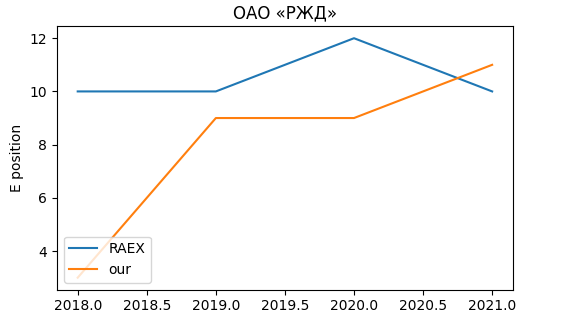
\includegraphics[width=0.8\linewidth]{images/E_ОАО «РЖД».png}
\caption{Сравнение E-рейтингов RAEX и TOPSIS для ОАО «РЖД». На графике видно, что тренды не похожи, но при этом в 2019-ом году и в середине 2020 позиции практически совпали.}
\label{fig:e_rgd}
\end{figure}

\begin{figure}[H]
\centering
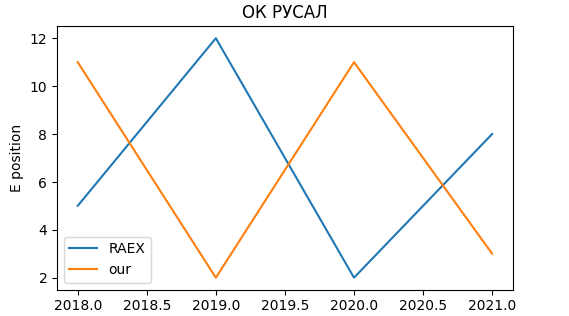
\includegraphics[width=0.8\linewidth]{images/E_ОК РУСАЛ.png}
\caption{Сравнение E-рейтингов RAEX и TOPSIS для ОК РУСАЛ. На графике видно, что тренды не похожи. Кажется, что есть смещение в данных, или в отчете РСПП отображена информация за предыдущий год, или рейтинг RAEX смотрит на данные за предыдущий год.}
\label{fig:e_rusal}
\end{figure}

\begin{figure}[H]
\centering
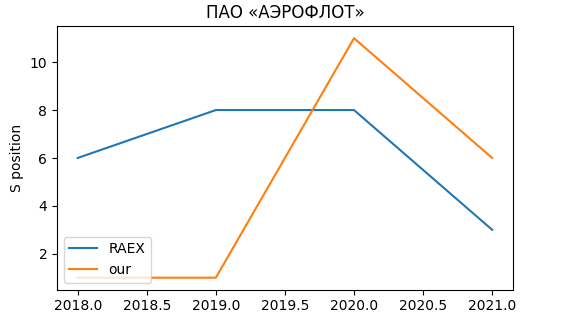
\includegraphics[width=0.8\linewidth]{images/S_ПАО «АЭРОФЛОТ».png}
\caption{Сравнение S-рейтингов RAEX и TOPSIS для ПАО «АЭРОФЛОТ». Тренды совпадают частично, в период с 2020-го по 2021 год, при этом абсолютные позиции разные.}
\label{fig:s_aeroflot}
\end{figure}

\begin{figure}[H]
\centering
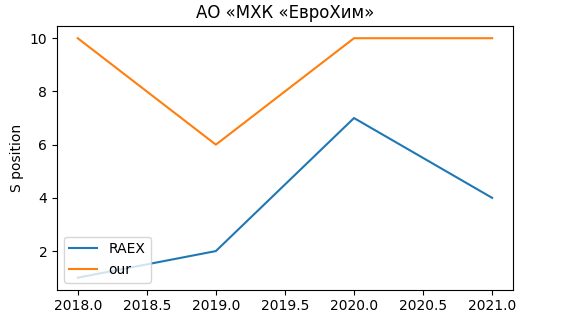
\includegraphics[width=0.8\linewidth]{images/S_АО «МХК «ЕвроХим».png}
\caption{Сравнение S-рейтингов RAEX и TOPSIS для АО «МХК «ЕвроХим». Тренды совпадают частично, в период с 2019-го по 2020 год, при этом абсолютные позиции разные.}
\label{fig:s_evrohim}
\end{figure}

\begin{figure}[H]
\centering
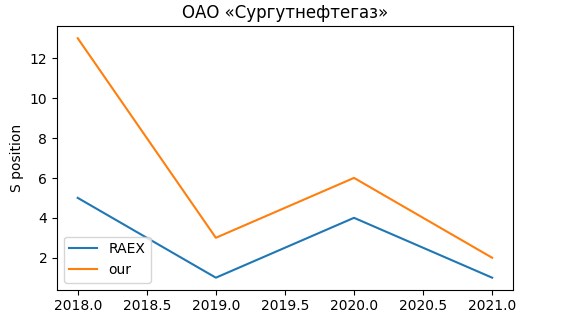
\includegraphics[width=0.8\linewidth]{images/S_ОАО «Сургутнефтегаз».png}
\caption{Сравнение S-рейтингов RAEX и TOPSIS для ОАО «Сургутнефтегаз». Тренды совпадают, при этом абсолютные позиции в каждом из рейтингов разные.}
\label{fig:s_surgutneftegaz}
\end{figure}

\begin{figure}[H]
\centering
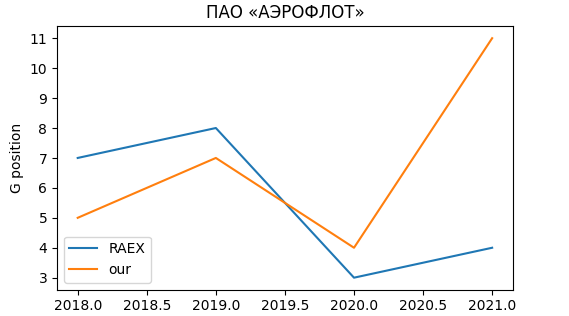
\includegraphics[width=0.8\linewidth]{images/G_ПАО «АЭРОФЛОТ».png}
\caption{Сравнение G-рейтингов RAEX и TOPSIS для ПАО «АЭРОФЛОТ». Тренды совпадают, при этом абсолютные позиции в каждом из рейтингов разные.}
\label{fig:g_aeroflot}
\end{figure}

\begin{figure}[H]
\centering
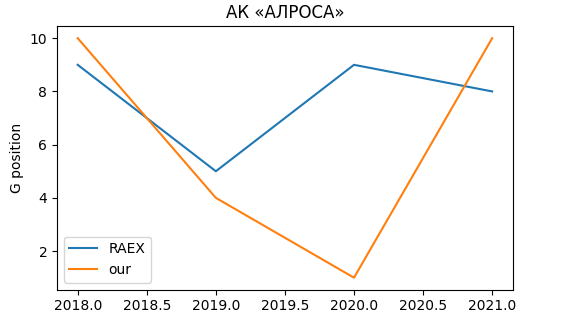
\includegraphics[width=0.8\linewidth]{images/G_АК «АЛРОСА».png}
\caption{Сравнение G-рейтингов RAEX и TOPSIS для АК «АЛРОСА». Тренды совпадают частично, возможно, что есть смещение в данных: и у RAEX и TOPSIS есть локальный минимум со сдвигом в один год, в 2019 и в 2020 году соответственно.}
\label{fig:g_alrosa}
\end{figure}

\begin{figure}[H]
\centering
\includegraphics[width=0.8\linewidth]{images/G_ПАО «ЛУКОЙЛ».png}
\caption{Сравнение G-рейтингов RAEX и TOPSIS для ПАО «ЛУКОЙЛ». Тренды совпадают, при этом абсолютные позиции в каждом из рейтингов разные.}
\label{fig:g_lukoil}
\end{figure}

\begin{figure}[H]
\centering
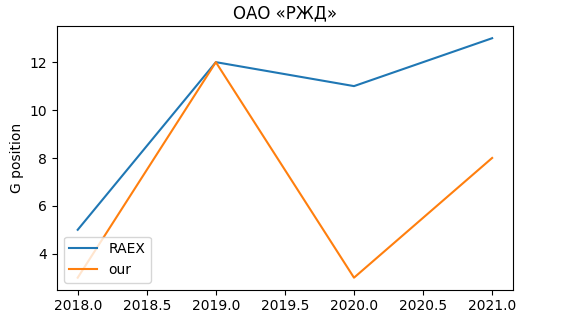
\includegraphics[width=0.8\linewidth]{images/G_ОАО «РЖД».png}
\caption{Сравнение G-рейтингов RAEX и TOPSIS для ОАО «РЖД». Тренды совпадают, при этом абсолютные позиции в каждом из рейтингов разные, есть совпадение только в 2019 году.}
\label{fig:g_rgd}
\end{figure}

\begin{figure}[H]
\centering
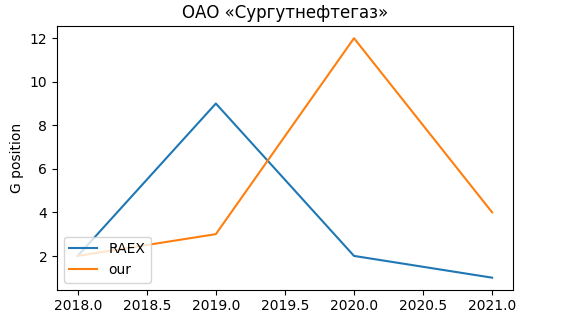
\includegraphics[width=0.8\linewidth]{images/G_ОАО «Сургутнефтегаз».png}
\caption{Сравнение G-рейтингов RAEX и TOPSIS для ОАО «Сургутнефтегаз». Тренды не похожи. Кажется, что есть смещение в данных, или в отчете РСПП отображена информация за предыдущий год, или рейтинг RAEX смотрит на данные за предыдущий год.}
\label{fig:g_surgutneftegaz}
\end{figure}

% \begin{figure}[H]
% \centering
% 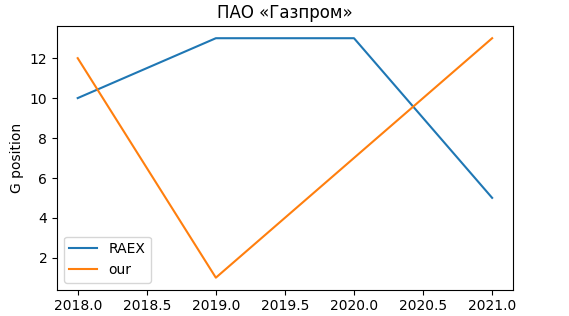
\includegraphics[width=0.8\linewidth]{images/G_ПАО «Газпром».png}
% \caption{Сравнение G-рейтингов RAEX и TOPSIS для ПАО «Газпром». Тренды полностью не совпадают, также как и абсолютные позиции.}
% \label{fig:g_gazprom}
% \end{figure}

Рассмотрим несколько примеров. На графиках (ось ординат --- позиция в рейтинге, ось абсцисс --- год) представлено изменения позиции компании согласно рейтингу RAEX и рейтингу, полученному нами на основе модели TOPSIS. На графике \ref{fig:e_rgd} тренды не совпадают, при этом рейтинги согласуются по позициям в 2019 году, а также в середине 2020-го года. На графиках \ref{fig:e_rusal}, \ref{fig:g_surgutneftegaz}, \ref{fig:g_alrosa} тренды не совпадают, при этом кажется, что есть сдвиг в данных, на основе которых составлялся один из рейтингов. Наример, при составлении отчета за 2020 год использовались данные 2019 года. На графиках \ref{fig:s_surgutneftegaz}, \ref{fig:g_aeroflot}, \ref{fig:g_lukoil}, \ref{fig:g_rgd} тренды рейтинга RAEX и полученного нами на основе нефинансовых отчетов совпадат, при этом абсолютные позиции разные. На графиках \ref{fig:s_aeroflot} и \ref{fig:s_evrohim} тренды свопадают частично, только в определнные периоды.

Также мы проверили есть ли корреляция между рейтингами, корреляция отсутствовала.

Расхождение в данных и остуствие корреляции можно объяснить тем, что рейтинговое агенство RAEX для составления своего ESG-рейтинга использует не только отчеты компаний, а всю доступную информацию --- 210 различных индикаторов, из которых 150 общих, остальные зависят от отрасли. Чтобы получить полноценный ESG-рейтинг, аналогичный рейтингу RAEX, к нашим данным нужно добавить информацию из новостей, сайтов компаний и т.д.

\subsection{Сравнение с Индексом РСПП «ОТВЕТСТВЕННОСТЬ
И ОТКРЫТОСТЬ»}

Для сравнения численного индекса, полученного нами на основе модели TOPSIS, с индексом РСПП «ОТВЕТСТВЕННОСТЬ
И ОТКРЫТОСТЬ» мы решили посмотреть какой диапазон значений принимает наш индекс для компаний соответстующих каждой букве из индекса «ОТВЕТСТВЕННОСТЬ И ОТКРЫТОСТЬ». Результаты оказались очень плохими: диапазоны для оценок «A» и «B» сильно пересекались, а в некоторые года максимум по знацениям TOPSIS-индекса для худшей оценки «B» даже превышал макимум оценки «A». Данный результат говорит о невозможности сопоставления рейтингов «ОТВЕТСТВЕННОСТЬ И ОТКРЫТОСТЬ» и полученного нами на основе модели TOPSIS.

Также мы пробовали другой подход для сопоставления двух индексов: решение задачи классификации, где признаками выступали факторы полученные нами после расчета косинусной близости, а таргетами были оценки «A» и «B» из индекса РСПП. Результаты классификации предствалены в таблице \ref{tab:t2}.
\begin{table}
    \begin{center}
        \begin{tabular}{ | l | c | c | c | c | c |}
        \hline
        Алгоритм & MSE & MAE & ROC-AUC & Accuracy & F1 \\ \hline
        CatBoost & 0.2 & 0.2 & 0.89 & 0.8 & 0.77 \\ \hline
        Random Forest & 0.17 & 0.17 & 0.86 & 0.83 & 0.8 \\ \hline
        AdaBoost Classifier & 0.33 & 0.33 & 0.67 & 0.67 & 0.58 \\ \hline
        Linear SVM & 0.2 & 0.2 & 0.79 & 0.8 & 0.77 \\ \hline
        RBF SVM & 0.47 & 0.47 & 0.10 & 0.53 & 0.0 \\ \hline
        Multilayer perceptron & 0.23 & 0.23 & 0.76 & 0.76 & 0.74 \\ \hline
        Logistic Regression & 0.27 & 0.27 & 0.74 & 0.73 & 0.73 \\ \hline
        \end{tabular}
        \caption{Результаты классификации}
        \label{tab:t2}
    \end{center}
\end{table}

Лучше всего себя показала модель CatBoost, но при такой маленькой выборке в первую очередь стоит обратить на более простые модели вроде логистической регрессии и метода опорных векторов, которые тоже неплохо себя показали.

\section{Заключение}

В результате выполнения данного проекта был получен поэтапный процесс по предобрабокте нефинансового отчета компании, выделения из него признаков и преобразования их в индекс ESG. На основе данного решения не получится получить полную оценку, так как в нефинансовых отчетах нет большой части информации, которую можно взять из других источников. Но можно использовать данный процесс, как основу для построения полноценного индекса.
\newline
Исходный код проекта лежит на платформе GitHub:
\newline
\href{https://github.com/MichaelYashchenko/ESG-Project}{https://github.com/MichaelYashchenko/ESG-Project}

\section{Дальнейшие шаги}

Данный проект имеет много направлений для дальнейшего исследования. Рассмотрим некоторые из них:
\begin{itemize}
    \item Использование всех топиков, выделенных Top2Vec, для классификации, чтобы модели самостоятельно выделяли значимые признаки. Но тут опять встает проблема с размером выборки.
    \item Использование других методов, помимо косинусной близости, для оценки схожести множества слов.
    \item Увеличение выборки за счет ручной разметки отчетов. Если собрать больше отчетов и разметить их по одной из методик, можно будет попробовать классифицировать тексты с помощью более мощных моделей, например BERT.
\end{itemize}

\newpage
 
% даём указание на включение данного место в оглавление как секции (\section)
\addcontentsline{toc}{section}{Список литературы}
 
%далее сам список используевой литературы
\begin{thebibliography}{}
    \bibitem{link:top2vec}  \href{https://arxiv.org/abs/2008.09470}{Dimo Angelov. Top2Vec: Distributed Representations of Topics // Computation and Language, August 2020.}
    \bibitem{link:tzentrobank} \href{http://www.cbr.ru/Content/Document/File/144085/Consultation_Paper_17012023.pdf}{Модельная методология ESG-рейтингов // Банк России, Доклад для
общественных консультаций, 2023.}
    \bibitem{link:rspp-methodik}  \href{https://rspp.ru/upload/content/909/1oii9yidubx9wteo5jemy7f89925nd5j/Metodika_2022.pdf}{Методика составления индексов РСПП по устойчивому развитию (ESG-Индексов), 2022.}
    \bibitem{link:raex-methodik} \href{https://www.raexpert.eu/files/Methodology_ESG_Corporates_V3.pdf}{Methodology for Assigning Environmental, Social and Governance Ratings to
Corporates // RAEX Europe, Frankfurt am Main, September 2019.}
\end{thebibliography}

% https://bpm.hse.ru/Runtime/Runtime/Form/AP__f__Request/?&itrequestid=1202295
% https://hse.antiplagiat.ru/report/byLink/apiCorp/577117?v=1&userId=4&validationHash=9C1D2EB84541260AEAB6B20CDB548641A105C97C&page=1


\end{document}
